\documentclass[12pt]{scrreprt}

\linespread{1.25}

\usepackage[ngerman]{babel}
\usepackage[utf8]{inputenc}
\usepackage{color}
\usepackage[a4paper,lmargin={4 cm},rmargin={2 cm},
tmargin={2.5 cm},bmargin = {2.5 cm}]{geometry}
\usepackage{amssymb}
\usepackage{graphicx}
\usepackage{pdfpages}
\usepackage{hyperref}

\begin{document}
	
\begin{titlepage}
		
	\includepdf[scale=1]{TitelblattBA}
		
\end{titlepage}	
	
\newpage
\tableofcontents
\newpage
	
\listoffigures
\addcontentsline{toc}{chapter}{Abbildungsverzeichnis}
\newpage
	
\listoftables
\addcontentsline{toc}{chapter}{Tabellenverzeichnis}
\newpage
	
\chapter{Einleitung}
Es war schon immer die Frage ob Maschinen jemals selbst, anhand vorhandenen Informationen, Entscheidungen treffen oder wie ein Mensch Regeln aus bestimmten Prozessen extrahieren können \cite{Chollet2018}(K.1.1.1). Diese Fragestellung ist vor allem in der heutigen Zeit, in der das Thema Digitalisierung voran getrieben wird, von großer Bedeutung. Auch setzen Unternehmen immer mehr auf Techniken aus dem Bereich des Maschinellen Lernens (ML) und verwenden diese um ihre Prozesse zu digitalisieren und somit zu optimieren. Es existieren verschiedene ML-Techniken, wie zum Beispiel die Klassifikation, Regression oder Deep Learning. Letzteres steht im Mittelpunkt vieler Anwendungsszenarien. Anwendungsfelder für Deep Learning sind vor allem, Bild- und Videoanalyse, sowie die Sprachverarbeitung. Diese werden in verschiedenen Branchen, wie zum Beispiel der Medizin, der Automobilindustrie oder im Kundendienst eingesetzt \cite{FraunhoferGesellschaft2018}. Auch im Bereich Online-Retail finden ML-Techniken einen relevanten Einsatz. Im Rahmen dieser Bachelor-Arbeit liegt der Fokus vor allem in diesem Bereich und wie die Bildanalyse hier unterstützten kann. Diese Problemstellung wird in einem späteren Abschnitt der Arbeit näher definiert.  \\
	\\
Diese Bachelor-Arbeit beinhaltet die Erkennung von Objekten auf Bildern durch den Einsatz von Künstlicher Intelligenz. Dabei wird die Disziplin Deep Learning unter Einsatz von Convutional Neural Network verwendet. Um diese zu verstehen werden allgemeine Informationen zur Künstlichen Intelligenz und dessen Bestandteile und Algorithmen benötigt. Zu Beginn ist es wichtig zu wissen, welche Probleme die Künstliche Intelligenz lösen kann und welche Bestandteile für diese Arbeit benötigt werden. In diesem Zusammenhang wird zum Beispiel das Verfahren Convutional Neural Network behandelt, welches zu den Deep Learning Methoden gehört und eine Teilmenge der Maschinellen Lernalgorithmen bildet. Außerdem wird im Rahmen dieser Arbeit das CRIPS-DM Modell vorgestellt und verwendet, welches als Standard für Data Mining Modelle definiert wurde.
	
\newpage
\chapter{Maschinelles Lernen}
	
Maschinelles Lernen stellt ein Teilgebiet der Künstlichen Intelligenz dar. Dabei werden durch den Einsatz von Maschinen ein Verhalten aus den Daten extrahiert, wodurch die Maschine selbst Lernen kann. Dies Geschieht unter Verwendung verschiedener Techniken und Algorithmen. Während der Lernphase versucht die Maschine, Regelmäßigkeiten aus den Daten zu erkennen und diese zu verallgemeinern. Nachdem die Lernphase beendet ist, kann die Maschine eine Vorhersage aus den aktuellen Daten treffen \cite{Frochte2021}(S.2-3).
	\\
\begin{figure}[h!]
	\centering
	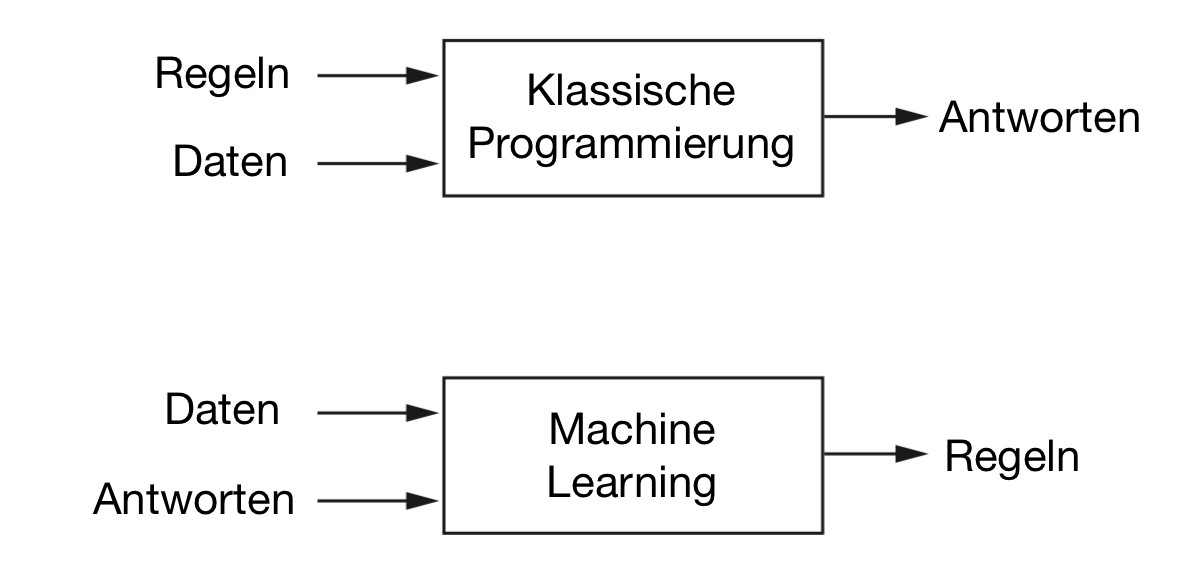
\includegraphics[width=12cm, height=5cm]{Abbildung_MaschinellesLernen_1.jpg}
	\caption{Maschinelles Lernen vs. Klassische Programmierung \cite{Chollet2018}(K.1.1.2}
	\label{fig:fig1}
\end{figure}
\\
In der Abbildung \ref{fig:fig1}, ist der Unterschied zwischen der Klassischen Programmierung und den Maschinellen Lernalgorithmen zu sehen. Bei der Klassischen Programmierung werden Regeln definiert und implementiert. Anhand dieser Regeln werden die Daten verarbeitet, die dann zu einer Antwort führen. Anders ist es aber bei den Maschinellen Lernalgorithmen. Hier werden Daten und dessen Antworten als Eingabedaten betrachtet, wodurch die Maschine für sich die Regeln definiert \cite{Chollet2018}(Kapitel 1). Dazu haben alle Maschinelle Lernverfahren zwei Phasen. Die erste Phase ist die Lernphase, in der es lernt, aus den Eingabedaten ein Muster zu extrahieren. Nachdem diese Phase beendet ist, wird die Anwendungsphase gestartet. Diese Phase wird sowohl für die Evaluation des Künstliche Intelligenz als auch für die Anwendung genutzt. Es ist zu beachten das die Künstliche Intelligenz auch in der Anwendungsphase lernen kann  \cite{Chollet2018}(Kapitel 2.1). 
\\
\\
Um Entscheidungen zu treffen, werden Eingabedaten benötigt, die der Maschine die nötigen Informationen liefern. Die Eingabedaten beinhalten auch die Lösung des Problems und somit auch den Wert, der von der Maschine vorhergesagt werden soll. Damit die Maschine nach Effizienz bewertet werden kann, ist eine Messung der Algorithmen erforderlich \cite{Chollet2018}(Kapitel 1.1.3).
\\
\\
Für die Lösungen der Probleme werden verschiedentliche Maschinelle Lernalgorithmen verwenden. Die Entscheidung welches benutzt werden soll hängt von den Eingabedaten und dem Ziel ab. Im Rahmen dieser Arbeit liegt der Fokus auf dem Convutional Neural Network Verfahren, welches zur Kategorie des überwachten Lernens gehört \cite{Luber2019}.
\section{Überwachtes Lernen}
Das überwachte Lernen gehört zu den Lernverfahren des maschinellen Lernens und umfasst die Klassifikation und Regression. Bei einem überwachten Lernen werden Eingabedaten, die Beispiele beinhalten, einem bekannten Zielwert zugeordnet. Dadurch sind die Zielwerte bekannt und somit können die Fehler, bei einer falschen Klassifikation, während dem Lernprozess entdeckt werden \cite{Chollet2018}(K.4.1.2).
	
\section{Künstliche Neuronale Netze}
	
Im folgenden Abschnitt werden die Bestandteile von künstlichen Neuronalen Netzen definiert und der Aufbau beschrieben.
	
\subsection{Neuronales Netz}\label{chapter:NeuronalesNetz}
	
Auf der linken Seite der Abbildung \ref{fig:fig2}, befinden sich die Eingabedaten die als $x_{0}, x_{1}, ..., x_{n} \in{\vec{X}}$  definiert sind, wobei $\vec{X}$ den Vektor $\mathbb{R}^n$ darstellt. Jede einzelnen Eingabe $x_{0}, x_{1},...,x_{n}$ wird mit seinem Gewicht $w_{n,j}$ multipliziert, wobei $j \in{[0,Anzahl Neuronen]}$ gilt. Nachdem multiplizieren mit den Gewichten werden alle berechneten Werte an die Übertragungsfunktion übergeben. Dieser Ablauf ist dabei an eine echte Nervenzelle angelehnt, indem Neuronen aus anderen Nervenzellen, dieses Neuron anregen und auf diese übertragen können. Die Übertragungsfunktion summiert diese Werte zusammen und leitet sie dann an die Aktivierungsfunktion weiter. Die Aktivierungsfunktion beinhaltet genauso ein Schwellenpotenzial mit der wir auch Schwellenwerte prüfen können. Eine einfache Aktivierungsfunktion wäre hierbei das Alles-oder-nichts-Prinzip. Mit diesem Prinzip ist gemeint, dass bei Überschreitungen des Schwellwertes das Neuron aktiviert und unterhalb des Schwellwertes inaktiv gestellt wird \cite{Frochte2021}(S.169).
\\
\begin{figure}[h!]
	\centering
	\includegraphics[width=10cm,height=5cm]{Abbildung_NeuronaleNetze_1.png}
	\caption{Modell eines Neurons \cite{Abbildung2}}
	\label{fig:fig2}
\end{figure}

Zunächst ist wichtig wie die Vernetzungen und Verknüpfungen der Neuronen aussehen und funktionieren. In Abbildung \ref{fig:fig3} wird deutlich, dass ein einfaches Künstliches Neuronales Netz aus drei Schichten besteht. Die erste Schicht ist dabei die Eingabeschicht (engl. Inputlayer), die die Eingabe der Daten verarbeitet und wiederum mit jedem Neuron aus der verborgenen Schicht (engl.= Hiddenlayer) vernetzt ist. Durch die Ausgabeschicht werden Regeln, die aus der verborgenen Schicht extrahiert werden, bereitgestellt. Diese Neuronen werden zur Evaluation des Modells benutzt \cite{Frochte2021}(S.169).
	
\begin{figure}[h]
	\centering
	\includegraphics[width=8.5cm,height=6cm]{Abbildung_NeuronaleNetze_2.jpg}
	\caption{Schichten der Künstliche Neuronale Netze \cite{Abbildung3}}
	\label{fig:fig3}
\end{figure}
	
\subsection{Feed-Forward Propagierung}
	
Das neuronale Netz durchläuft bei jedem Dateineintrag einmal alle Schichten. Verwendet wird dafür, dass im Abbild \ref{fig:fig2} vorgestellte Modell.
	
\subsubsection{Mathematische Beschreibung eines Feed-Forward Netzes}
	
In den vorherigen Abschnitten wurden die Bestandteile und deren Funktionen näher erklärt. An dieser Stelle wird das einfache neuronale Netz beschrieben. Dafür wird zuerst die Arbeitsweise zwischen den Schichten definiert:
	
\begin{center}
	$f: \mathbb{R}^{D_{0}} \to \mathbb{R}^{D_{l}}$ , $f(\overrightarrow{X})$ = $(f_{l} \circ f_{l-1} \circ ... \circ f_{1})(u)$,
\end{center}
	
wobei $f_{l}$ die Schichten sind und für jedes L $\in$ \{ $0, 1, 2, ..., l$ \} die Funktion,\\
	
\begin{center}
	$f: \mathbb{R}^{D_{L-1}} \to \mathbb{R}^{D_{0}}$ , $f_{l}(\overrightarrow{X}) = \phi (w^{l} * \overrightarrow{X} + b^{l} ) $, beschreibt.
\end{center}
	
Wobei $\overrightarrow{X}$ der Vektor für die Eingabedaten (engl. Inputdata), $w^{l}$ $\in$ $\mathbb{R}^{(D_{l} \times D_{l-1})}$ die Gewichte, welche die Verbindungen (Abbild \ref{fig:fig3}) von einem Neuron zu anderen Neuronen gewichten und $b^{l}$ der Verzerrungsvektor (engl. Bias), der Schicht l ist. $\phi$ ist die Aktivierungsfunktion der Schicht \cite{Plaue2021} (S.232 - 234).\\
\\
\subsubsection{Lern- und Testphase}
	
Während der Lernphase wird das Model mit einer teil menge von den gesamte Daten, gefüttert. Durch dies wird das Model trainiert, daher nennt man diese Phase auch Trainingsphase. Damit keine Informationen aus der gesamten Datenmenge durchsickern, werden nur die Trainingsdaten in das Model gefüttert. Damit das Model während der Trainingsphase bewertet werden kann, benötigt es eine Mengen an Daten aus den gesamte Datensatz, die  als Validierungsmenge an das Model übertragen wird. Somit stellt sich fest das bei der Bewertung eines Modells, damit anfängt die gesamt Daten in Trainigs-, Validierungs- und Testdaten zu verteilen  \cite{Chollet2018} (K.4.2.1).\\
	
\begin{figure}[h!]
	\centering
	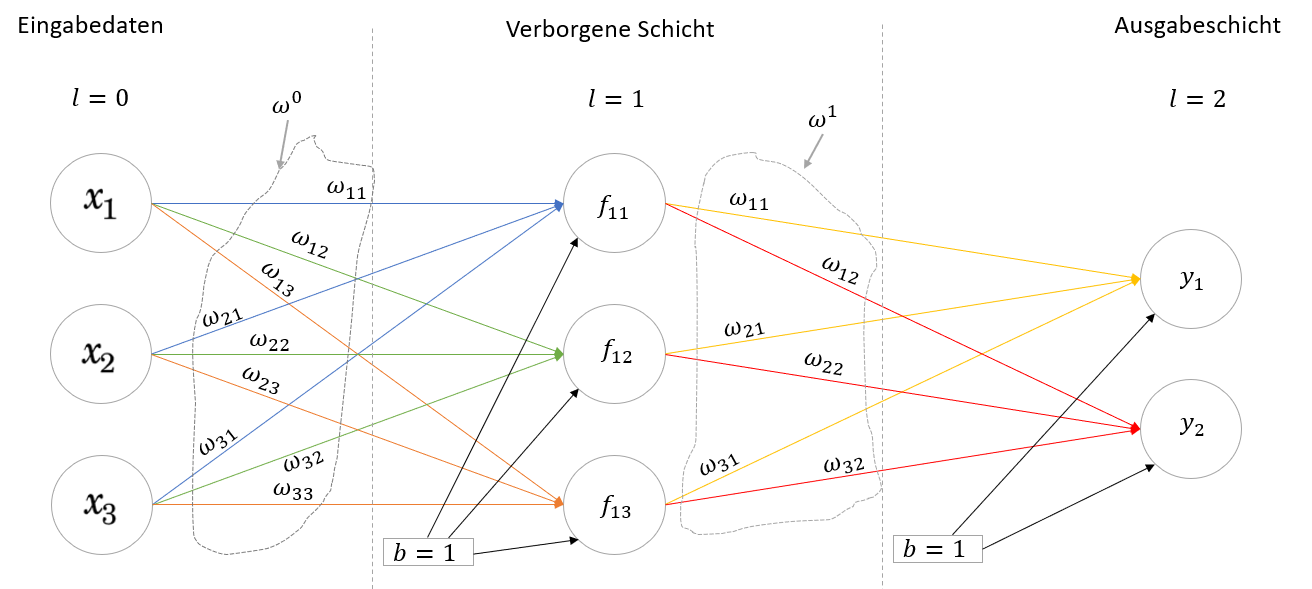
\includegraphics[width=15cm,height=6cm]{FF_Netz.png}
	\caption{Feed-Forward Netz \cite{Halil2022}}
	\label{fig:fig10}
\end{figure}
	
Die Gewichte werden zunächst zufällig vergeben und mit dem Lernverfahren, das während der Rückpropagierung stattfindet, optimiert. Damit das Neuronale Netz Abweichungen erkennen kann, werden Bias verwendet, die diese Abweichung darstellten. Bevor mit der   Trainingsphase begonnen wird, sollten folgende Elemente festgelegt werden. Zunächst ist die Verlustfunktion zu definieren, welche die Leistung der Trainingsdaten beschreibt. Durch die Verlustfunktion kann das Neuronale Netz die Gewichte optimieren. Als nächstes sollte die Menge an Trainingsdaten und Testdaten festgelegt werden \cite{Chollet2018} (K.2.1 Listing 2.2). An dieser Stelle werden beispielhaft die Schritte der Feed-Forward Propagation in Abbild \ref{fig:fig10} betrachtet. Zunächst wird die Eingabeschicht mit den Eingabedaten gefüttert, wobei diese normalisierte Werte beinhalten sollten. Die zufällig generierten Gewichte stellen die Gewichtungen für die Neuronen der nächsten Schicht dar. Nun wird das, in Abbild \ref{fig:fig10} definierte, Model für jedes Neuron aus der nächsten Schicht angewendet. Somit hat das erste Neuron aus der Schicht l=1  folgende Berechnung. 
	
\begin{center}
	$f_{11} =  \phi [(x_{1}* w_{11}) +( x_{2}* w_{21}) + (x_{3}* w_{31})]  + b^{1}$
\end{center}
	
allgemein lässt sich die Feed-Forward Propagierung wie folgt beschreiben:
	
\begin{center}
	$f = \sum^{n}_{n=0} [ \phi (x_{n} * w_{nj} + b^{j})]$
\end{center}
	
, wobei n die Anzahl an Neuronen im vorherigen Schicht sind und j die Anzahl an Neuronen im aktuellen Schicht. Somit kann das Neuronale Netz mit den bestmöglichen Gewichten Prognosen anhand Eingabedaten, liefern. Die Optimierung der Gewichte wird im Abschnitt \ref{chapter:Lernverfahren} Lernverfahren näher beschrieben.\\
	
\subsection{Eingabedaten}
Die Eingabedaten $x_{1}, ..., x_{n}$ stellen die Merkmale (oder Attribute) dar, welches die Eigenschaften beinhalten, aus denen das Neuronale Netz lernen kann. Zu beachten sind dabei die Datentypen der Eingabedaten und die Normierung dieser Daten. Dabei gibt es unterschiedliche Datentypen. Im Rahmen dieser Arbeit ist der Fokus auf Vektor- und Bilddaten gerichtet \cite{Chollet2018} (K.2.2.8). 
	
\subsubsection{Vektordaten}
	
Dieser Datentyp wird mathematisch als $ \overrightarrow{x} \in \mathbb{R}^{2}$ definiert und beinhaltet in der ersten Achse, die Datenwerte, wie zum Beispiel $x_{1}$. Die zweite Achse ist die Merkmalsachse, welche die Merkmale darstellt die zur Verfügung stehen  \cite{Chollet2018} (K.2.2.9).
	
\subsubsection{Bilddaten}
	
Bei den Bilddaten handelt es sich generell um drei dimensionale Matrizen, jedoch unterscheiden wir die Graustufenbilder, für diese zwei Dimensionale Matrizen ausreichen. Hier bekommt jeweils eine Achse die Höhe, die zweite Achse die Breite und die letzte Achse die Farbtiefe des Bildes. Da die Graustufenbilder nur einen Farbkanal beinhalten, ist die zwei dimensionale Matrix ausreichend \cite{Chollet2018} (K.2.2.11).
	
\subsection{Lernverfahren}\label{chapter:Lernverfahren}
Bisher wurde der Durchlauf eines Neuronalen Netzes definiert, jedoch nicht wie es aus den Daten lernen kann. Damit das Neuronale Netz lernen kann, muss er auch Fehler erkennen können. Abhängig von der Verlustfunktion ist auch die Aktivierungsfunktion, die für die Ausgabeschicht ausgewählt wurde. Je nach Größe oder Art der Ziel-Klassen wird eine Aktivierungsfunktion ausgewählt. Ein Beispiel dazu ist die Mehrfachklassifizierung, bei der die Aktivierungsfunktion "Softmax" ausgewählt wird. Die Softmax-funktion auch als Softmax-Regression bekannt, stellt anhand der Eingabewerte eine Wahrscheinlichkeitsverteilung zu Verfügung, deren Summe 1 ergibt. Somit werden den Ziel-Klassen werte vergeben die zwischen 0 und 1 sind \cite{Mahmood2018}. Durch die Vereinheitlichung der Neuronen mit der Aktivierungsfunktion, können Fehlerwerte kalkuliert werden. Dies Geschieht folgendermaßen. Es wird angenommen, dass die Ausgabeschicht den Wert $x_{0} = 0.75$ beinhaltet, wobei der echte erwartete Wert y = 1 ist. Durch die Anwendung  eines der Verlustfunktionen, stellt das Neuronale Netz fest, wie groß die Abweichung des Ergebnisses von dem tatsächlichen Ergebnis ist. Hierzu werden unterschiedliche Verfahren genutzt  \cite{Matzka2021}(S.124-126). Eines dieser Verfahren ist die mittlere quadratische Abweichung (engl. mean squared error, MSE).
	
\begin{center}
	\centering
	$MSE = \frac{1}{n} (\sum\limits_{i=1}^{n})(Y_{i} - \hat{Y_{i}})^{2}$
\end{center}
	
, wobei n Anzahl der Datenpunkte, $Y_{n}$ das erwartete Ergebnis und $\hat{Y_{i}}$ die prognostizierten Werte sind.\\
	
In diesem Beispiel wird es wie folgt berechnet.
	
\begin{center}
	$MSE = \frac{1}{1} \sum\limits_{i=1}^{1}(Y_{i} - \hat{Y_{i}})^{2}$\\
	
	$MSE = 1 * (1 - 0.75)^{2} = 0.0625$\\
\end{center}
	
Somit kennt das Neuronale Netz die Abweichung der Prognose, womit es den Lernprozess starten kann. Es stellt sich die frage wie das Neuronale Netz sich optimieren bzw. verbessern lässt. \cite{Plaue2021} (S.194).  Es ist bekannt das ein Neuronales Netz mehrere Ausgaben liefern kann und für jeder dieser Ausgaben ist es möglich eine Verlustfunktion zuzuweisen. \cite{Chollet2018}.
	
\subsubsection{Verlustfunktion}
	
Die Verlustfunktion (engl. loss-, costfunktion) wird in der Optimierung während der Trainingsphase genutzt. Hierzu gibt es Verschiedentliche Funktionen wie zum Beispiel der oben genannte mittlere quadratische Abweichung. Ein anderes Beispiel, ist die Cross-Entropy-Loss Funktion, welches für die Optimierung von klassifikatorische  modele geeignet ist. Die Cross-Entropy-Loss Funktion ist ähnlich wie die Softmax Funktion aufgebaut. Sie misst den Abstand zwischen den Prognostizierten Wert und den Wahrheitswert, um so nah wie möglich in die richtige Richtung des Ergebnisses zu bewegen. Während der Trainingsphase werden die Gewichte iterativ und entsprechend mit dem Ziel, den Cross-Entropy-Loss zu minimieren, angepasst \cite{Mahmood2018}. Im Rahmen dieser Arbeit wird die Cross-Entropy-Loss Funktion angewendet, da es sich um eine mehrfachklassifizierung handelt.
	
\subsubsection{Rückpropagierung}
	
Die Anpassung der entsprechende Gewichte wird durch den Rückpropagierung ermöglicht. Damit die Gewichte angepasst werden können, ist es nötig das das Model Fehlerwert ein Minimum annimmt. Es ist bekannt das mit dem Gradienten der Funktion das Minimum erreichbar ist, welches die partielle Ableitung aller Vektoren darstellt. Dieser Vektor wird auch $\delta(f)$ genannt. Sie zeigt an jedem Punkt der Funktion, die Richtung der steilsten anstieg  (bzw. maximum), wobei  $-\delta(f)$ die Richtung der steilsten abstieg (bzw. minimum) der Funktion zeigt \cite{Vogl2021} (S.337). Allgemein wird der Gradientenverfahren folgendermaßen definiert:\\
	
\begin{center}
	$x^{i+1} = x^{i} - \eta * \delta(f(x^{i}))$
\end{center}
	
, wobei $x^{0}$ der Startpunkt ist und $\eta$ die Schrittweite. Diese Verfahren lässt sich wie folgt bei den Gewichten integrieren.
	
\begin{center}
	$w_{neu} = w_{alt} - \eta * \delta (E(W_{alt}))$
\end{center}
	
, wobei w das Gewicht darstellt und $\eta$ die Schrittweite.\\
\\
Somit kann das Neuronale Netz seine Gewichte anpassen, womit es sich optimieren kann. Der Ablauf zu Anpassung der Gewicht wird folgendermaßen definiert.


TODO:
ABLAUF DES RÜCKPROPAGIERENS MUSS DEFINIERT WERDEN !
	
	
	
	
	
	
	
	
	
	
	
\section{Deep Learning}
	
Bei Deep Learning handelt es sich um eine Teilmenge der Maschinellen Lernalgorithmen, mit der komplexere Aufgaben gelöst und automatisiert werden können. Der Unterschied zu einem Künstlichen Neuronalen Netz ist, dass Deep Learning mehrere verborgene Schichten beinhaltet (siehe Abbildung \ref{fig:fig4}). Hierzu ist die Aktivierungsfunktion als die Sigmoid-Funktion vorgesehen, die wie folgt definiert ist:
	
\begin{center}
	$sig(t) = \frac{1}{(1 + e^-t)}$\\
\end{center}
	
,wobei $sig(t) \in [0,1]$ und $ t \in \mathbb{R}$ gilt. 
\\
	
Dies bedeutet, dass die Neuronen immer eine Zahl übertragen bekommen, die zwischen 0 und 1 liegt. Somit können durch Implementierungen Schwellenwerte definiert und dementsprechend Neuronen aktiviert oder deaktiviert werden \cite{Frochte2021}(S.178).\\
	
\begin{figure}[h!]
	\centering
	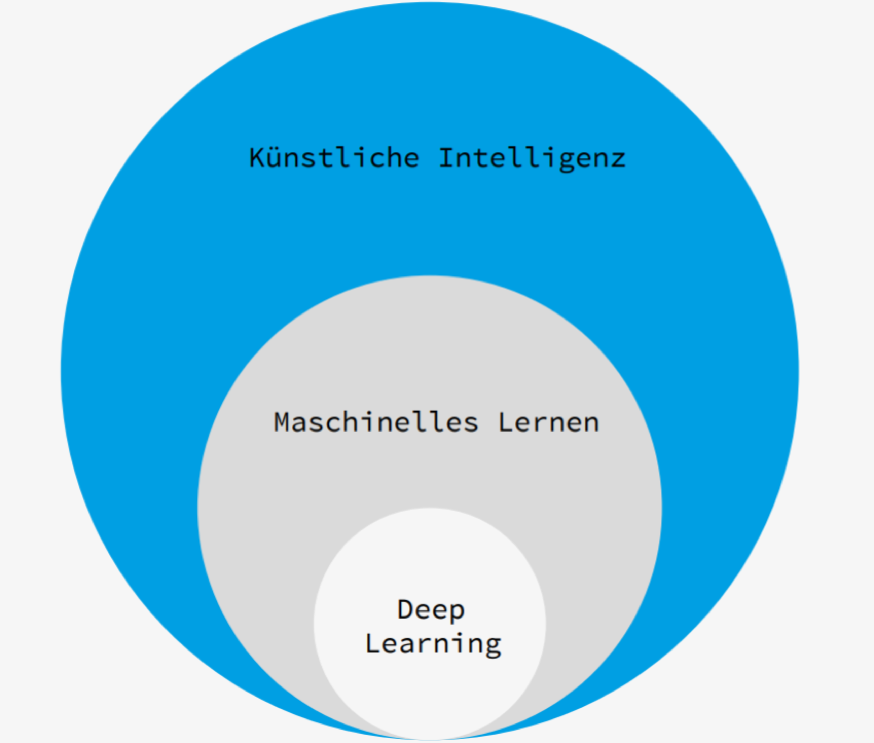
\includegraphics[width=13cm,height=7cm]		{Abbildung_DeepLearning_1.jpg}
	\caption{Künstliches Neuronales Netz vs. Deep Learning \cite{Abbildung4}}
	\label{fig:fig4}
\end{figure}
	
\subsection{Convolutional Neural Network}
	
Bei einem CNN, im Deutschen "gefaltetes Neuronales Netzwerk", handelt es sich von einer Sonderform des künstlichen neuronalen Netzes, das speziell für Bild- oder Audiobearbeitung entwickelt wurde. Diese Form ist teils an den biologischen Ablauf angelehnt.\cite{Luber2019} Der Aufbau eines CNNs ist in Abbildung \ref{fig:fig5} dargestellt.
	
\begin{figure}[h!]
	\centering
	\includegraphics[width=13cm,height=5cm]		{Abbildung_CNN_1.png}
	\caption{Aufbau eines CNNs \cite{Abbildung5}}
	\label{fig:fig5}
\end{figure}
	
In Abbildung \ref{fig:fig5} sind mehrere Schichten (Layer) zu sehen. Dabei ist die Eingabeschicht (Inputlayer) und die Ausgabeschicht (Outputlayer) bekannt. Wie im vorherigen Abschnitt auch definiert, hat ein CNN mehrere verborgene Schichten, darunter den \textbf{Convolutional Layer}, der einzelne Merkmale aus den Eingabedaten ortsunabhängig erkennt und daraufhin diese extrahiert. Diese Merkmale könnten bei einer Bildverarbeitung den Kanten, Linienformen und Farbtupfer entsprechen, die eine Struktur darstellen. Diese Merkmale werden in der \textbf{Pooling-Schicht}, auch als Subsampling bekannt, bearbeitet, indem die Auflösung der Merkmale reduziert und verdichtet wird. Somit werden überflüssige Informationen verworfen, wodurch die Datenmenge reduziert wird. Dadurch wird die Berechnungsgeschwindigkeit erhöht. Diese zwei Schichten können so oft wie möglich verwendet werden, da sie nur Merkmale aus den Bilder extrahieren und optimierend zu Verfügung stehen. Die eigentliche Klassifikation entsteht durch den \textbf{Fully-Connected Layer}, im Deutschen "vollständig verknüpfte Schicht", der sich der wiederholten Abfolge der Convolutional- und Pooling-Schichten anschließt, indem alle Merkmale der vorgelagerten Schichten mit jedem Ausgabemerkmal verknüpft sind. Somit werden mögliche Kombinationen aus den Strukturen entworfen, die komplexere Strukturen identifizieren lassen. Wichtig ist hierbei, dass die Anzahl an Neuronen in der vollständig vernetzten Schicht abhängig von den Klassen oder Objekten sind \cite{Luber2019}. 
	
\section{Evalutionstechniken}

TODO:
Genauigkeit definieren und wie dies zustanden kommt? Was stellt es dar?








\newpage
\chapter{CRISP-DM Modell}
	
Das CRISP-DM Modell "Cross-Industry Standard Process for Data Mining" beschreibt den Standard für die Strukturierung der Maschinellen Lernalgorithmen. Das Ziel ist es, einen einheitlichen Prozess für Data Mining Projekte zu schaffen und ist eine Anleitung für Data Mining, die in 6 Schritten aufgeteilt ist \cite{Wuttke}. Der Ablauf des Modells ist in Abbildung \ref{fig:fig6} dargestellt.
	
\begin{figure}[h!]
	\centering
	\includegraphics[width=9cm,height=8cm]		{Abbildung_CRISP_DM_1.png}
	\caption{Ablauf CRIPS-DM Modell \cite{Abbildung6}}
	\label{fig:fig6}
\end{figure}
	
\subsubsection{Business Understanding}
	
Der erste Schritt der 6 Schritte des CRISP-DM Modells, ist das Business Understanding, welches sich mit den betriebswirtschaftlichen Problemen befasst. Zunächst werden betriebswirtschaftliche Anforderungen extrahiert und analysiert, wodurch die Grundlagen für weitere Schritte und Entscheidungen gebildet werden. Damit ein Verständnis über die betriebswirtschaftlichen Fragestellungen übermittelt wird, ist es wichtig die Anwender in die Data Mining Prozesse mit einzubeziehen.\\
	
Das Business Understanding beinhaltet 4 Aspekte, die in Betracht gezogen werden sollen. Hierzu gehört wie zuvor auch erwähnt, die Bestimmung der betriebswirtschaftlichen Problemstellungen und dessen Zielkriterien. Ein weiterer Aspekt, ist die Situationsbewertung, welches die zur Verfügung gestellten Ressourcen für das Data Mining Projekt beschreibt. Dies bedeutet zum Beispiel die Software- und Personalressourcen. Zusätzlich werden Risiken, die, während dem Data Mining Projekt entstehen können, identifiziert. Auch die Bestimmung analytischer Ziele ist ein Aspekt des Business Understanding, indem eine Analyse der zuvor bestimmten betriebswirtschaftlichen Probleme durchgeführt wird. Auch Erfolgskriterien für das Data Mining Projekt werden bestimmt, wie zum Beispiel eine Optimierung des Geschäftsprozesses um 5\% mit weniger Bedarf an Ressourcen. Der letzte Aspekt beinhaltet die Erstellung des Projektplans, welches die beabsichtigten Ziele des Projektes beschreibt, indem die Auflistung der einzelnen Schritte mit jeweiliger Zeitspanne definiert werden. Hinzu kommen die möglichen Risken oder Ursachen für das Scheitern des Projektes, die aufgefasst werden.
	
\subsubsection{Data Understanding}
	
In diesem Schritt werden relevante Datenbestände, die zu einer Hypothese führen können, aufgestellt. Zum Beispiel werden bei einer Wettervorhersage die aktuellen Zustände der Atmosphäre betrachtet. In diesem Fall ist der Datenbestand die Zustände der Atmosphäre. Zunächst werden Daten gesammelt, die benötigt werden und zu einer bereits bestehenden Datenmenge integriert. Als nächstes werden diese Datenbestände beschrieben. Hierzu werden Eigenschaften wie Quantität, Formateigenschaften, Anzahl der Einträge und Felder der Daten erfasst. Der letzte Schritt des Data Understanding ist die Untersuchung und die Bewertung der Daten, in dem eine Analyse mit den Daten betrieben wird, um erste Hypothesen und Erkenntnisse zu treffen und diese dann zu dokumentieren. Bei der Bewertung der Daten wird sichergestellt, dass die Daten verwendbar sind und sie keine fehlende Attributwerte enthalten \cite{Wuttke}.
	
\subsubsection{Data Preparation}
	
Um die finale Menge der Datenauswahl zu erstellen, wird der Schritt Data Preparation durchgeführt. An erster Stelle werden Daten ausgewählt, die für das Ziel des Projektes relevante Informationen hergeben. Wichtig hierbei ist zu betrachten, dass die Daten in dem richtigen Datenformat gespeichert werden \cite{Wuttke}.
	
\subsubsection{Modeling}
	
Um eine vorliegende Problemstellung aus dem Bereich Maschinelles Lernen lösen zu können, stehen verschiedene Modelle beziehungsweise Algorithmen zur Verfügung. Aus diesen Modellen wird dann das Model ausgesucht, welches im Bezug zum definierten Ziel das optimale Ergebnis liefert. Manche Modelle benötigen hierzu vorbestimmte Datenstrukturen, die dazu führen können, einen Schritt zurück zu gehen und sich noch einmal mit der Datenvorbereitung zu befassen. Anschließend wird das Modell trainiert und getestet um die Qualität und Genauigkeit des Modells zu überprüfen \cite{Wuttke}.
	
\subsubsection{Evaluation}
	
Vor der Finalisierung des Data Mining Projektes, ist es noch notwendig zu prüfen, ob die Qualität des Modelles für das Ziel des Projektes ausreicht. Ist das Ergebnis noch nicht gut genug oder werden vorher definierte Ziele nicht erreicht, müssen die Gründe für das Scheitern analysiert und entsprechende Änderungen im Modell vorgenommen werden. Dies hat zufolge, dass die vorherigen Schritte nochmals durchlaufen werden müssen \cite{Wuttke}.
	
\subsubsection{Deployment}
	
Als letztes werden die aus dem erstellten Modell gewonnen Erkenntnisse für die Nutzer vorbereitet und ihm als Anwendung zur Verfügung gestellt. Damit kann ein Anwender zum Beispiel eigene Daten in das Modell hochladen und erhält, je nach der vorliegenden Problematik, ein Ergebnis für seine verwendeten Daten \cite{Wuttke}.
	
\newpage
\chapter{Experimente}
	
\section{Business Understanding}
	
Online-Versandhändler haben oft eine hohe Rückläuferquote. Diese Rückläuferquote kommt zum Beispiel durch den Kauf von Artikeln in verschiedenen Größen zustande. Die nicht passenden Größen werden dann vom Käufer wieder zurückgesendet. Unter diese Versandhändler fällt, mit einer Rückläuferquote von bis zu 50\%, auch das Unternehmen Zalando. Dabei müssen 97\% der zurückgesendeten Produkte wieder eingelagert und verkauft werden \cite{Hoefer2018}. Für den erneuten Verkauf werden die Produkte, in diesem Betrachtungsfall Klamotten, identifiziert, gelabelt und bei Bedarf wieder eingelagert. Das Unternehmen Zalando verschickte im Jahr 2019 rund 186 Millionen Bestellungen \cite{Rabe2021}. Wenn man davon ausgeht, dass eine Bestellung 4 Artikel beinhaltet und 50\% der Bestellungen wieder zurückgesendet werden, ergibt das 372 Millionen Artikel, die wieder neu gelabelt und eingelagert werden müssen.\\
	
Die Unterstützung und Optimierung der Rückläuferbearbeitung, kann zum Beispiel durch eine AI gestützte Klassifikation gewährleistet werden. Mit diesem Ansatz kann dann die zu einem Artikel zugehörige Kategorie, auf Basis von Bildern, bestimmt werden. Damit ergibt sich die Frage- bzw. Problemstellung, inwiefern können Machine Learning Algorithmen bei der Klassifizierung von Bildern einzelner Kleidungsstücke unterstützen?
	
\section{Data Understanding}
	
Der für diese Arbeit gewählte Datensatz heißt Fashion MNIST und wurde im Jahr 2017 von dem Unternehmen Zalando veröffentlicht. Der Datensatz steht in einer GitHub Repository zur Verfügung und ist frei zugänglich \cite{Zalando2017}. Er beinhaltet Zalando-Artikelbilder, die in zwei Datensätze aufgeteilt sind. Der erste Satz enthält 60.000 Beispiele, die für das Training verwendet werden und der zweite Satz 10.000 Beispiele, die für das Testen verwendet werden. Jedes Beispiel, welches jeweils ein Bild darstellt, ist ein 28x28 Graustufenbild. Jedem Bild wird dabei noch ein Label zugeordnet. Ein Label repräsentiert eins der 10 Klassen, wobei jede Klasse eine Artikelkategorie darstellt. In der folgenden Abbildung \ref{fig:fig7} ist eine Übersicht des Datensatzes bzw. der Bilder zu sehen. Dabei werden pro Klasse drei Zeilen beansprucht.\\
	
\begin{figure}[h!]
	\centering
	\includegraphics[width=15cm,height=15cm]		{Abbildung_DatensatzAlsBild.jpg}
	\caption{Der gesamte Datensatz: FASHION-MNIST \cite{Abbildung7}}
	\label{fig:fig7}
\end{figure}
	
Der ursprüngliche MNIST Datensatz, der durch Fashion-MNIST ersetzt wurde, ist sehr beliebt und wird oft verwendet, um Algorithmen zu validieren. Es heißt auch „If it doesn't work on MNIST, it won't work at all". Jedoch wurde der MNIST Datensatz aufgrund seiner Einfachheit ausgetauscht \cite{Zalando2017}.\\
	
Auch die Labels bestehen aus 28x28 Pixeln, wobei jeder einzelne Pixel einen Wert zwischen 0 und 255 annehmen kann. Der aktuelle Datensatz Fashion-MNIST enthält folgende 10 Klassen bzw. Labels:
	
\begin{table}[h!]
	\begin{center}
		\begin{tabular}{|c|c|c|}
			\hline
			Label & Artikel \\
			\hline
			0 & T-shirt/top \\
			\hline
			1 & Trouser \\
			\hline
			2 & Pullover \\
			\hline
			3 & Dress \\
			\hline
			4 & Coat \\
			\hline
			5 & Sandal \\
			\hline
			6 & Shirt \\
			\hline
			7 & Sneaker \\
			\hline
			8 & Bag \\
			\hline
			9 & Ankle boot \\
			\hline
		\end{tabular}
		\caption{Labels des Datensatzes}
		\label{tab:labels}
	\end{center}
\end{table}
	
\newpage 
	
Der Trainings- als auch der Testdatensatz ist ziemlich ausgeglichen. In jedem Satz ist jede Kategorie mit ca. 10\% vertreten, was in den nächsten Abbildungen zu sehen ist.
	
\begin{figure}[h!]
	\centering
	\includegraphics[width=9cm,height=8cm]		{Abbildung_StatistikVerteilungTrainDatensatz.jpg}
	\caption{Verteilung Trainingsdatensatz \cite{Abbildung8}}
	\label{fig:fig8}
\end{figure}
	
\begin{figure}[h!]
	\centering
	\includegraphics[width=9cm,height=8cm]		{Abbildung_StatistikVerteilungTestDatensatz.jpg}
	\caption{Verteilung Testdatensatz \cite{Abbildung9}}
	\label{fig:fig9}
\end{figure}
\newpage
	
Aufgrund der Ausgeglichenheit der Daten müssen im Rahmen der Data Preparation keine großen Änderungen oder Vorbereitungen vorgenommen werden.
	
\section{Data Preparation}

Um die vorliegenden Daten für die modellierten ML-Verfahren verwenden zu können, müssen diese entsprechend vorbereitet werden. 

\subsection{Test- und Trainingsdaten}
Für die Vorbereitung werden die Trainingsdaten nochmal aufgeteilt. Dabei werden aus den vorhandenen 60000 Trainingssätzen, 6000 für die Validierung extrahiert. Dadurch bleiben für die Trainingsphase 54000 Datensätze übrig. Die Testdatensätze bleiben mit der ursprünglichen Anzahl von 10000 gleich.

\subsection{Skalierung der Merkmale}

Die Skalierung von Merkmalen dient zur Normalisierung des Bereichs der erklärenden bzw. unabhängigen Variablen. Das Verfahren ist auch als Datennormalisierung bekannt und wurde im Rahmen der Datenvorbereitung auf den Daten angewendet. Die Eingabedaten liegen als Graustufenbilder vor und besitzen Werte zwischen 0 und 255. Um die Normalisierung dieser Daten vorzunehmen, werden die Werte durch 255 geteilt um somit Ausprägungen zwischen 0 und 1 zu erreichen. 

\subsection{Datentransformation}

In dem Ausgangsdatensatz stellt jede Zeile mit seinen 784 Spalten, die wiederum als 28x28 Pixel zu verstehen sind, jeweils ein Bild dar. Für die spätere Verwendung der Daten, müssen diese aber umgeformt werden. Die Umformung der Graustufenbilder muss so erfolgen, dass ein Bild durch 28 Zeilen und 28 Spalten dargestellt wird und so die Pixel wiedergibt. Dadurch kann das Neuronale Netz eine genaue Position der Pixel identifizieren. Die dafür verwendete Methode kann dem beigefügten Notebook entnommen werden. Im Rahmen der Datentransformation werden außerdem die Zielvariablen in die vorhandenen 10 Kategorien unterteilt.

\section{Modellierung}

Insgesamt werden drei verschiedene implementierte Modelle vorgestellt und im nächsten Abschnitt evaluiert. Jedes Modell bzw. Experiment beinhaltet dabei ein Convolutional Neuronal Network. Die Unterschiede der drei Modelle liegen dabei in den verwendeten Schichten und deren Zusammenspiel. 

\subsection{Experiment 1}

Das erste implementierte CNN-Modell beinhaltet folgende drei Layer, die in vorherigen Abschnitten bereits erläutert wurden:

\begin{itemize}
	\item Convolutional Layer (Conv2D)
	\item Pooling Layer (MaxPooling2D)
	\item Flatten Layer (Flatten)
	\item Fully-Connected Layer (Dense)
\end{itemize}

Der Conv2D und MaxPooling2D Layer gehören, wie in Kapitel 2 beschrieben, zu dem Feature-Extraktor. Die beiden Schichten werden zwei mal nacheinander in das Modell integriert. Im Anschluss werden dem Modell zwei Dense Layer hinzugefügt. Der erste Conv2D Layer bekommt die Eingabedaten im 28x28 Pixel Format, daher erhält diese Schicht einen Input-Parameter, der die Dimension der Eingabedaten beschreibt. Im MaxPooling2D werden die aus den Conv2D extrahierten Merkmale in eine 14x14 dimensionale Matrix zusammengefasst. Der zweite Conv2D Layer erhält nach dem MaxPooling2D Layer Daten in der Form 14x14 Pixeln, aus dem der Layer dann wiederum Merkmale extrahiert. Der anschließende MaxPooling2D Schicht fasst diese Merkmale dann nochmals zusammen. Als nächstes formt der Flatten Layer die Merkmale in eine eindimensionale Matrix um. Zuletzt folgen dann die beiden Dense Layer. Die erste Dense Schicht ist der Fully-Connected Layer und die zweite eingesetzte Dense Schicht der Output Layer (Ausgabeschicht). Der ersten Dense Schicht wird dabei die Aktivierungsfunktion Recitifier übergeben. Die Recitifer (relu) wird wie Folgt definiert.

\begin{center}
	$f(x) = max(0,x)$, wobei x der Eingangswert ist.
\end{center}

... . Für die Ausgabeschicht wird die Aktivierungsfunktion softmax eingestellt. Damit wird das erste Modell finalisiert und kann trainiert werden.

\begin{figure}[h!]
	\centering
	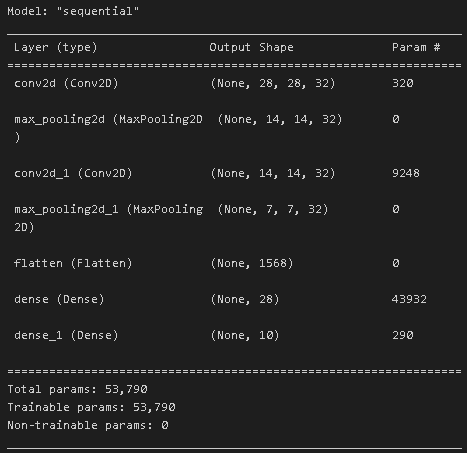
\includegraphics[width=15cm,height=10.5cm]		{ExperimentModelAufbau_1.png}
	\caption{  Modellaufbau \cite{HK22} (Experiment 1)}
	\label{fig:fig13}
\end{figure}

Insgesamt kann das Model 53,790 Parameter trainieren. Bevor das Training gestartet werden kann, müssen noch einige Variablen definiert werden. Zunächst braucht das Modell ein optimizer der ein tensorflow Objekt darstellt. Dieses Objekt beschreibt den Optimierung Vorgang für das Modell. In diesem Fall wird der optimizer als "tf.keras.optimizers.Adam()" definiert, der den stochastische Gradientenabstiegsverfahren beschreibt. Der nächste Parameter definiert die Verlustfunktion des Modells, welches wir als Cross-Entropy-Loss Funktion angeben. Als Bewertungsmetrik wird dem Modell die Genauigkeit (engl. accuracy) ausgewählt, die Prozentual angibt wie gut ein Modell prognostiziert. Zu letzte werden Epochen-Anzahl und Batch-Größen angegeben. 

\subsubsection{Trainingsphase}

 Mit dem Fitten der Trainings- und Validierungsdaten wird die Trainingsphase gestartet. Nachdem die Trainingsphase beendet ist werden Bewertungsmetriken genutzt um eine Darstellung der Leistung des Modells zu bekommen.

\begin{figure}[h!]
	\centering
	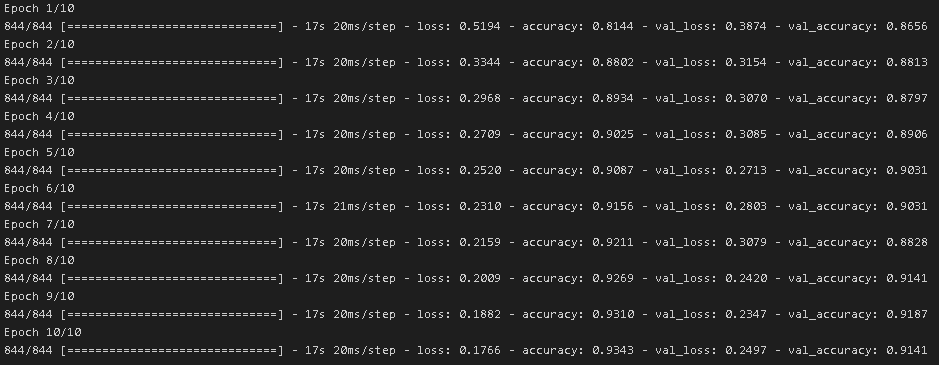
\includegraphics[width=14.5cm,height=10cm]		{ExperimentModelTrainingsphase_1.png}
	\caption{ Bewertung Trainingsphase \cite{HK22}(Experiment 1)}
	\label{fig:fig14}
\end{figure}

Die Ergebnisse zeigen, das die erste Epoche eine Genauigkeit von $86,56\%$ hat und die sich bei den nächste Epoche erhöhen. Damit hat das Model am ende eine Genauigkeit, während dem Training von $91\%$. Sichtbar ist die Differenz zwischen accuracy ($93,34\%$) und $val\_accuracy$ ($91,14\%$). Die accuracy (auch Genauigkeit genannt) beschreibt in diesem Fall, die Genauigkeit der Trainingsdaten, diese wird jedoch nicht für die Bewertung genutzt. Die $val\_accurac$, welches die Genauigkeit der Validierungsdaten anzeigt wird hier in Betracht gezogen, da diese zu Validierung des Modells erstellt worden ist und komplett abgekapselt von den Trainingsdaten übergeben wurde. Der nächste Schritt zu Optimierung des Modell, sollte die Anpassung sein, welches den Abstand der Genauigkeiten verringert. Es ist auch ersichtlich, dass die loss-Werte gegen null näher. Dies Zeigt, dass das Modell sich verbessert bzw. optimiert. Die Leistung können wir auch anhand eines Graphen bilden indem, die Ergebnisse in Epoche aufgeteilt und  geplotten werden, dies wird folgendermaßen Dargestellt.\\
\\
\\
\begin{figure}[h!]
	\centering
	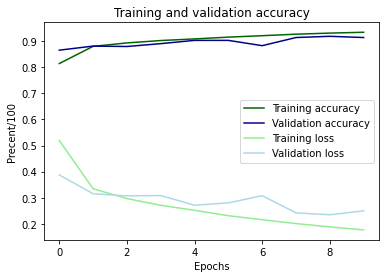
\includegraphics[width=15cm,height=9cm]		{ExperimentModelBewertungsgraf_1.png}
	\caption{ Bewertung Trainingsphase anhand Graphen \cite{HK22}(Experiment 1)}
	\label{fig:fig15}
\end{figure}

In diesem Abbild wird die Verbesserung des Modell durchaus ersichtlicher. Es ist klar deutlich das sich die loss-Werte gegen null näher, währenddessen die Genauigkeit sich erhöht. Somit wird das Modell immer weiter optimiert bis zur letzten Epoche.

\subsection{Experiment 2}

In diesem Experiment wird das Modell aus dem Experiment 1 übernommen und weiter verbessert. Das Ziel ist zunächst die reduzierung der Differenz von $val\_accuracy$ und accuracy, damit das Modell genauere Bewertung liefern kann. Dafür wird die Dropout Schicht benutzt, welches die Daten eliminiert, die ein Ausreißer bilden.

 

\cleardoubleoddpage
	
\addcontentsline{toc}{chapter}{Literaturverzeichnis}
\bibliography{Literatur}
\bibliographystyle{alpha}
	
\cleardoublepage
	
\end{document}